\documentclass[11pt, titlepage]{article}

\usepackage{wasysym}
\usepackage{caption}
\usepackage{amsmath}
\usepackage[subpreambles]{standalone}
\usepackage{graphicx}
\graphicspath{ {./images/} }

\usepackage{hyperref}
\hypersetup{
	colorlinks=true,     
    urlcolor=blue,
    linkcolor=black
}

\usepackage{geometry}
\geometry{margin=1in}

\begin{document}
\title{RAM Robotic Test Leg}
\author{by Christopher Mailer (MLRCHR001)}
\maketitle


\tableofcontents

\newpage
\section{Design Calculations}
\subsection{Specifications}
\begin{itemize}
	\item T-Motor U10 Plus 80KV
	\item Coaxial 5 bar linkage leg design
	\item Place to attach foot designs
	\item Components purchased from RS Components
	\item Use of 2:1 timing belt for lightweight quasi-direct-drive actuation
\end{itemize}

\subsection{T-Motor U10 Plus 80KV}
\begin{table}[h]
\centering
\caption*{Motor Properties}
\begin{tabular}{ l l }
\hline
 Pole Pairs & 21 \\
 Weight & $405\,g$ \\
 Internal Resistance & $135\,m\Omega$ \\
 Startup Torque & 7.5\,Nm \\
 Max Rated Speed & $4000\,rpm$ \\
 Max Continuous Current & $25\,A$ \\
 Max Continuous Power & $1200\,W$ \\\hline
\end{tabular}
\end{table}

\subsection{Timing Belt Selection}
\subsubsection{Profile and Pitch}
The 'T' timing belt profile was chosen as it is a standard profile providing the largest selection of belts and pulleys on RS Components.\newline
The selected timing belt pitch type of T5 was minimum pitch which would support transmission of the 1.2\,kW of power produced by each of the motors while still providing a large selection of belt sizes on RS Components. Additional considerations were that a larger pitch such as the T10 pitch would be accompanied by a larger belt width, thus increasing the overall size of the design. A smaller pitch such as the T2.5 on the other hand would be challenging to accurately 3D print the pulley tooth profile.

\subsubsection{Material}
The predominant T5 timing belt type on RS Components was the polyurethane CONTI SYNCROFLEX with steel tension members. Polyurethane belts have better abrasion resistance than rubber belts.

\newpage
\subsection{Small Pulley Sizing}
Based on the dimensions of the motor and pulley mounting interface, the smallest pulley pitch diameter which can be mounted to the motor while still accommodating the mounting bolts is $\diameter 36$.

\begin{equation}
	z_1 = \frac{d_1\cdot \pi}{t} = \frac{(36)(\pi)}{5} = 22.62\,teeth
\end{equation}

The next available standard number of pulley teeth  is 24 resulting in the following tooth pitch

\begin{equation}
	d_1 = \frac{z\cdot t}{\pi} = \frac{(24)(5)}{\pi} = 38.20\,mm	
\end{equation}

The centre to centre distance of the small and large pulleys is currently unknown but could be estimated to be approximately 90\,mm, thus allowing the number of engaged teeth on the small pulley to be estimated

\begin{equation}
	z_e = z_1 (0.5-\frac{d_2-d_1}{2\pi C}) = (24)(0.5-\frac{(2)(38.20)-38.20}{(2)(\pi)(90)}) \approx11
\end{equation}

\subsection{Timing Belt Width}
The small pulley is the limiting component in the calculating of the timing belt width as it is where maximum tooth shear is experienced.

\begin{table}[!h]
\centering
\caption*{Belt Specific Tooth Strength at 4000\,rpm from datasheet}
\begin{tabular}{ l r r r l}\hline
		Specific Torque & $M_{spec}$ & = & 1.91 & Ncm/cm \\
		Specific Power & $P_{spec}$ & = & 3.81 & W/cm \\\hline
\end{tabular}
\end{table}

\begin{table}[!h]
\centering
\caption*{Given conditions}
\begin{tabular}{ l r r r l}\hline
	Power & $P$ & = & 1.2 & kW \\
	Torque & $M$ & = & 7.5 & Nm \\
	Number of Teeth & $z_1$ & = & 24 & Nm \\
	Teeth in Mesh & $z_e$ & = & 11 & teeth \\\hline
\end{tabular}
\end{table}

\subsubsection{Tooth Shear Strength}
Calculation of the belt width based on power
\begin{equation}
	b = \frac{10^4\cdot P}{z_1 \cdot z_e \cdot P_{spec}} = \frac{(10^4)(1.2)}{(24)(11)(3.81)} = 11.93\,mm
\end{equation}
Calculation of the belt width based on torque
\begin{equation}
	b = \frac{10^3\cdot M}{z_1 \cdot z_e \cdot M_{spec}} = \frac{(10^3)(7.5)}{(24)(11)(1.91)} = 14.87\,mm
\end{equation}
The next standard belt width which exceeds both of these is 16\,mm

\subsubsection{Tension Member Strength}
The maximum allowable tension for a T5 16\,mm wide timing belt is 570\,N
\begin{equation}
	F_u = \frac{2 \cdot 10^3 \cdot M}{d_1} = \frac{(2)(10^3)(7.5)}{38.20} = 393\, N < 570\,N
\end{equation}
Therefore the selected timing belt will be able to withstand the loads

\subsection{Timing Belt Length}
The centre to centre distance of the timing belt needs to be larger than 90\,mm to provide sufficient clearance between the pulleys, but should also be kept to a minimum to ensure a compact design.

\begin{table}[!h]
\centering
\caption*{Given conditions}
\begin{tabular}{ l r r r l}\hline
	Centre to centre distance & $C$ & $\ge$ & 90 & mm \\
	Small pulley no. of teeth & $z_1$ & = & 24 & teeth \\
	Large pulley no. of teeth & $z_2$ & = & 48 & teeth \\\hline
\end{tabular}
\end{table}

\begin{equation}
	d_i = \frac{z_i\cdot p}{\pi}
\end{equation}

\begin{equation}
	\theta_1 = 2\cdot\arccos(\frac{d_2-d_1}{2\cdot C}) = 2,71\,rad
\end{equation}

\begin{equation}
	\theta_2 = 2\pi -\theta_1 = 3,57\,rad
\end{equation}

\begin{equation}
	L = 2\cdot C\cdot \sin(\frac{\theta_1}{2}) + \theta_1\cdot\frac{d_1}{2} + \theta_2\cdot\frac{d_2}{2} = 364,07\,mm
\end{equation}

The next available standard timing belt length is 365\,mm which requires a centre to centre distance of 90,48\,mm.


\subsection{Selected Timing Belt}
CONTI SYNCROFLEX T5 Timing Belt, 73 teeth, 365\,mm length, 16\,mm width

\newpage
\subsection{Shaft Loading Condition}
The maximum forces experienced by each of the shafts will be during landing when the legs are fully extended and the force will be transmitted directly to the shafts and not shared by the motors as torque.

\subsubsection{Leg Impact Force}
Approximating the rubber pad on the base of the foot as a spring and assuming all of the gravitational potential energy is transferred to spring energy, the following can be determined:

\begin{equation}
	E_p = mgh
\end{equation}

\begin{equation}
	E_s = \frac{1}{2}k\delta^2
\end{equation}

\begin{equation}
	\delta = \sqrt{\frac{2E_p}{k}}
\end{equation}

The rubber pad on the base of the foot was approximated to have a spring constant of $30\times10^3\,N/m$. The test rails also only allow for a maximum jump height of 1\,m. The maximum ground reaction force experienced by the leg during landing is therefore;

\begin{equation}
	F_{max} = \sqrt{2mghk} = \sqrt{(2)(3)(9.81)(1)(30\times10^3)} = 1329\,N
\end{equation}

This is a conservative estimate as other means of energy dissipation are ignored. This force will be evenly distributed between each leg linkage producing 665\,N on the end of each shaft.

\subsubsection{Belt Tension}
Assuming belt tensioned to full capacity of $P_1 = 570\,N$
\begin{equation}
	P_2 = P_1-\frac{2M}{d_1} = 570 - \frac{(2)(7.5)}{0.0382} = 141.4\,N
\end{equation}

The centre to centre distance of timing belt pulleys, and therefore angle of wrap of the belts at this stage in the design is unknown. Instead the belts are conservatively assumed to be parallel, resulting in all of the tension being transmitted to the shaft.

\begin{equation}
	P_{res} = P_1 + P_2 = 711.4
\end{equation}

\subsubsection{Combined Load}
The legs will exert maximum force on the shaft during landing when in the fully contracted or extended states. In this case the impact force from the legs will be transmitted to the shaft almost directly upwards. The angle of the belt tensions is acting at $45^{\circ}$ to the vertical. The shaft is also expected to transmit 15\,Nm of torque after the 2:1 speed reduction from the motor.
\begin{table}[h!]
\centering
	\begin{tabular}{c c c}
		$P_{x}$ & = & 503\,N \\
		$P_{y}$ & = & 503\,N \\
		$M$ & = & 15\,Nm \\
	\end{tabular}
\end{table}

\newpage
\subsection{Inner Shaft BMD}
\noindent\textbf{Side View}
\begin{figure}[h]
\centering
	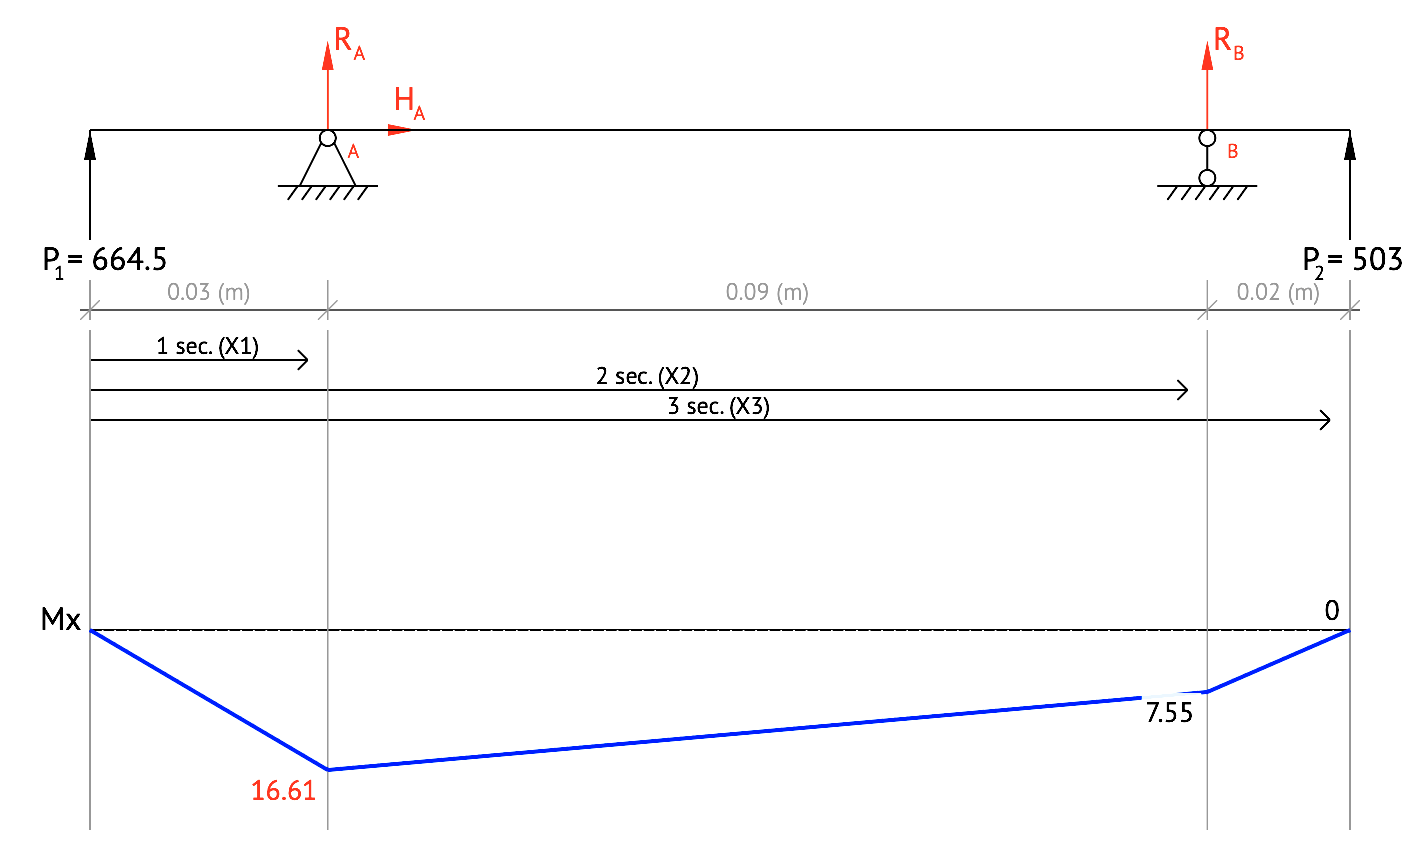
\includegraphics[width=10cm]{inner_shaft_side_bmd.png}
	\caption{Inner shaft side view bending moment diagram \href{beamguru.com/online/beam-calculator/?save=e3c807530bc8028842f255e179b1241b}{BeamGuru}}
\end{figure}

${R_{A}}_y = -762.53\,N$ \hfill
${R_{B}}_y = -404.97\,N$\hfill
$M_{xz}=16.61$\newline

\noindent\textbf{Top View}
\begin{figure}[h]
\centering
	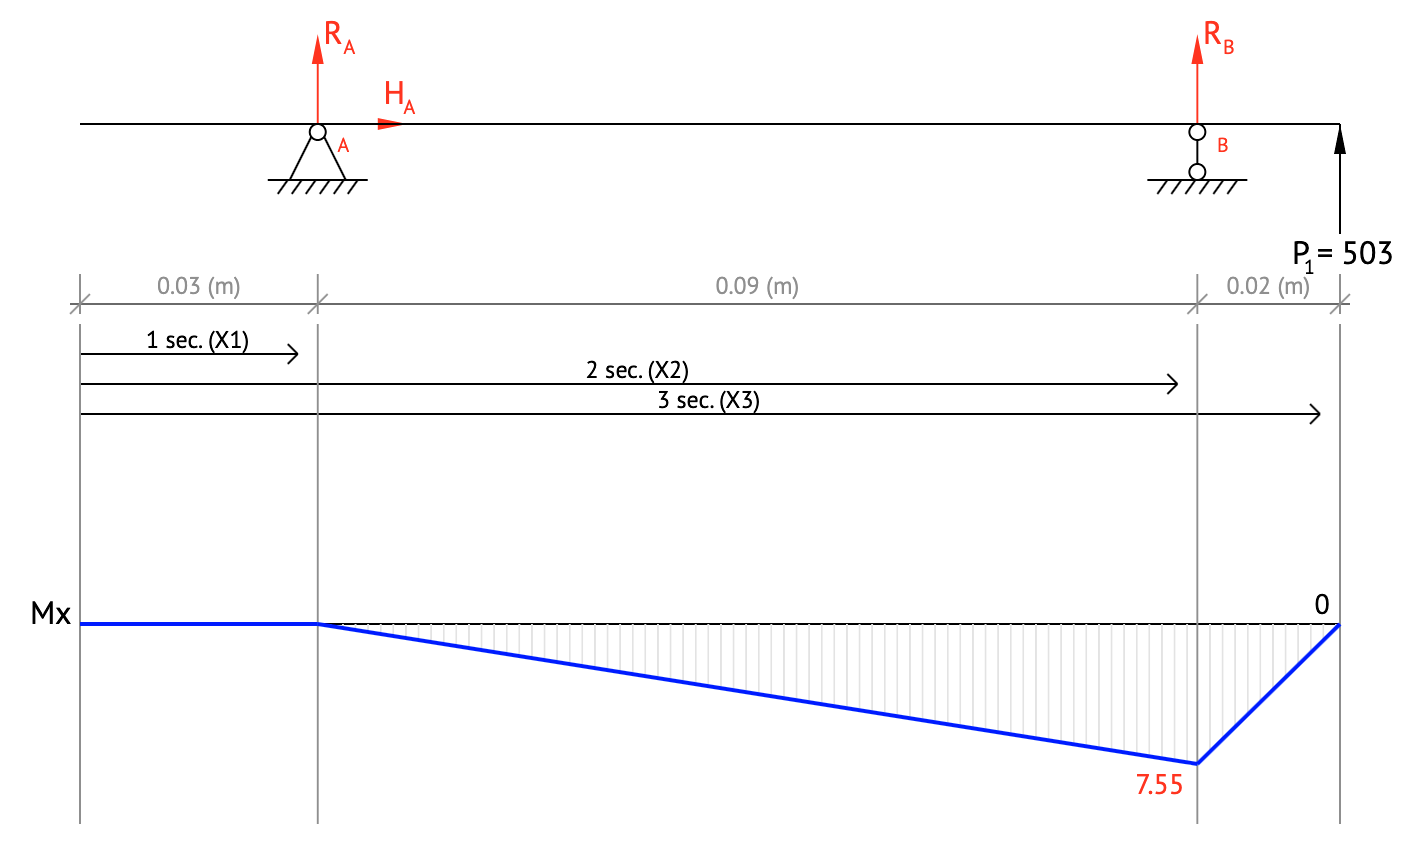
\includegraphics[width=10cm]{inner_shaft_top_bmd.png}
	\caption{Inner shaft top view bending moment diagram \href{beamguru.com/online/beam-calculator/?save=88759fc0e73600b1a941d8defae4d6b8}{BeamGuru}}
\end{figure}

${R_{A}}_x = 81.57\,N$ \hfill
${R_{B}}_x = -584.57\,N$\hfill
$M_{yz}=0$\newline

\noindent\textbf{Resultant}\newline
Critical section at leftmost bearing
$$M = \sqrt{{M_{xz}}^2 + {M_{yz}}^2} = 16.61\,Nm$$
$$T = 15\,Nm$$


\newpage
\subsection{Outer Shaft BMD}
\noindent\textbf{Side View}
\begin{figure}[h]
\centering
	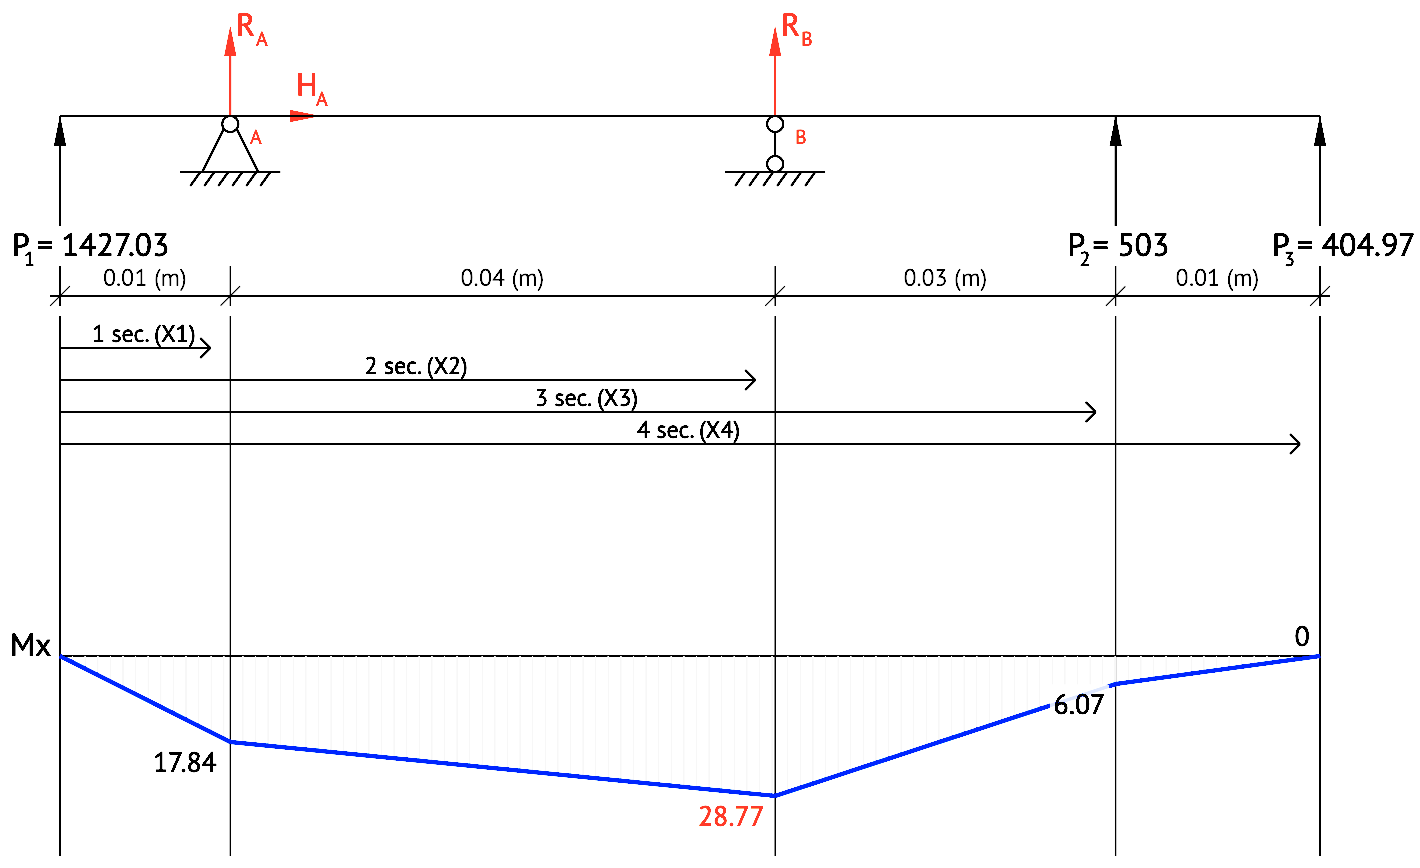
\includegraphics[width=10cm]{outer_shaft_side_bmd.png}
	\caption{Outer shaft side view bending moment diagram \href{beamguru.com/online/beam-calculator/?save=e3c807530bc8028842f255e179b1241b}{BeamGuru}}
\end{figure}

${R_{A}}_y = -1153.63\,N$ \hfill
${R_{B}}_y = -1181.37\,N$\hfill
$M_{xz}=28.77$\newline

\noindent\textbf{Top View}
\begin{figure}[h]
\centering
	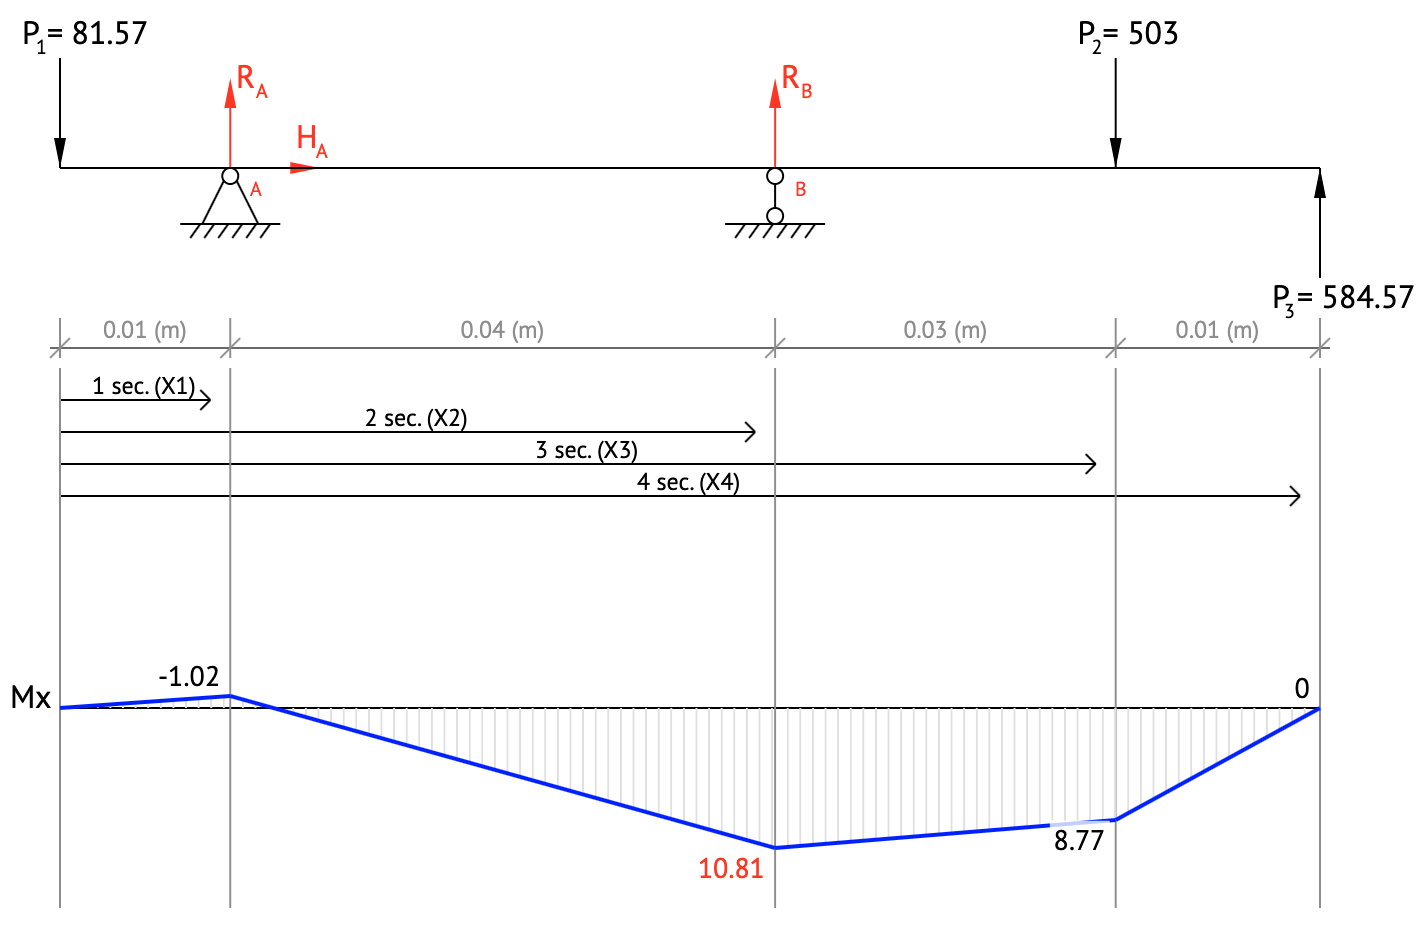
\includegraphics[width=10cm]{outer_shaft_top_bmd.png}
	\caption{Outer shaft top view bending moment diagram \href{beamguru.com/online/beam-calculator/?save=88759fc0e73600b1a941d8defae4d6b8}{BeamGuru}}
\end{figure}

${R_{A}}_x = 377.26\,N$ \hfill
${R_{B}}_x = -377.26\,N$\hfill
$M_{yz}=-1.02$\newline

\noindent\textbf{Resultant}\newline
Critical section at rightmost bearing
$$M = \sqrt{{M_{xz}}^2 + {M_{yz}}^2} = 30.73\,Nm$$
$$T = 15\,Nm$$

\subsection{Shaft Sizing}
\begin{equation}
	\sigma = \frac{Mr}{I} = \frac{32M}{\pi{d_o}^3(1-\frac{d_i}{d_0}^4)}
\end{equation}
\begin{equation}
	\tau = \frac{Tr}{J} = \frac{16 T}{\pi{d_o}^3(1-\frac{d_i}{d_0}^4)}
\end{equation}

\subsubsection{Material}
The shaft will be made from 304 Stainless Steel, as this was available in the workshop, thus the Maximum Distortion Energy Theory will be a sufficient failure theory.\newline\newline
$S_u = 215\,MPa$
\begin{equation}
	{\sigma_b}^2 + 3\tau^2 \le (\frac{S_u}{RF})^2
\end{equation}
The following calculations were done in the spreadhseet \textit{Shaft and Belt Calculations}

\subsubsection{Inner Shaft Size}
The Inner Shaft diameter selection was an iterative process driven by the Outer Shaft diameters and the available bearings on RS Components. A diameter of $\diameter12\,mm$ was selected as this provided a reserve factor of 1.7 and ensured a reasonable selection of roller bearings. A larger inner shaft would have resulted in a significantly larger outer shaft, greatly increasing the weight of the design.

$$D_o = 12\,mm$$
$$RF = 1,7$$

\subsubsection{Outer Shaft Size}
The outer diameter of the shaft was selected to be $\diameter20\,mm$ based on bearing availability on RS Components. With the goal of keeping size and mass to a minimum, the smallest roller bearings were selected which required the Outer Shaft to have an inner diameter of $\diameter16\,mm$. This produced a reserve factor of 3. To create a shoulder for the bearings, the remaining portion of the shaft has an inner diameter of $\diameter14\,mm$.

$$D_o = 20\,mm$$
$$D_i = 16\,mm$$
$$RF=3,0$$



\newpage
\section{Manufacture}
\subsection{3D Printing}

The following parts are 3D printed

\begin{table}[h]
\centering
\begin{tabular}{ l c}
	\textbf{Part Name} & \textbf{Qty} \\\hline
	Inner Timing Belt Gear & 1 \\
	Outer Timing Belt Gear & 1 \\
	Motor Mounting & 2 \\
	Support Brace & 1 \\
	Encoder Shaft & 2 \\
	Leg Spacer & 3 \\\hline
\end{tabular}	
\end{table}

\subsubsection{Printer Settings}
The Cura Ender 3 presets were used with the following modifications.

\begin{table}[h]
\centering
	\begin{tabular}{r l}
	\hline
		Printer & Ender 3 Pro\\
		Material & PLA \\
		Printing Temp. & $200^{\circ}$ \\
		Printing Speed & 50\,mm/s \\
		Layer Height & 0.2\,mm \\
		Infill Density & 60\% \\
		Infill Pattern & Cubic \\
		Adhesion Type & Raft \\
		\hline
	\end{tabular}
\end{table}

\subsubsection{Considerations}
The main challenge with 3D printed parts was shrinkage. To compensate holes were printed 4\% larger and reamed afterwards to remove seams. The shrinkage also resulted in the timing belt initially not being properly tensioned. New output pulleys were printed with 1\,mm larger outer diameters which corrected the problem.

\subsubsection{Additional Machining}
\begin{itemize}
	\item Holes need to be drilled out to remove seams
\end{itemize}


\newpage
\subsection{Laser Cutting}
The following parts are laser cut

\begin{table}[h]
\centering
\begin{tabular}{ l c c c}
	\textbf{Part Name} & \textbf{Material} & \textbf{Thickness} & \textbf{Qty} \\\hline
	Mounting Plate & 5182 Aluminium & 3\,mm & 1 \\
	Inner Short Leg Link & 5083 Aluminium & 10\,mm & 1\\
	Outer Short Leg Link & 5083 Aluminium & 10\,mm & 1 \\
	Extra Long Leg Link & 5083 Aluminium & 10\,mm & 1 \\
	Long Leg Link & 5083 Aluminium & 10\,mm & 1 \\
	\hline
\end{tabular}	
\end{table}

\subsubsection{Considerations}
Laser cutting thick material produces a rough edge and the cut does not remain perpendicular to the material surface. Thus, holes should be undersized before laser cutting and then later reamed to the correct size on a drill press to ensure a smooth finish and perpendicularity.

\subsubsection{Additional Machining}
\begin{itemize}
	\item The Mounting Plate requires sanding to remove rough edges
	\item The leg links require the bearing seats to be machined. This is a counterbore to a depth of 5\,mm. A cutting tool on a drill press achieves this.
	\item The holes for the shoulder bolts need to be drilled and tapped for the M5 shoulder bolt
	\item The holes for the inner and outer output shafts need to be reamed to the correct sizes
\end{itemize}








\newpage
\subsection{Machining}
The following parts were machined by the UCT workshop

\begin{table}[h]
\centering
\begin{tabular}{ l c c}
	\textbf{Part Name} & \textbf{Material} & \textbf{Qty} \\\hline
	Flange & 6082 Aluminium & 1 \\
	Motor Shaft (Short) & 6082 Aluminium & 1 \\
	Motor Shaft (Long) & 6082 Aluminium & 1 \\
	Inner Shaft & 304 Stainless Steel & 1 \\
	Outer Shaft & 304 Stainless Steel & 1 \\
	Timing Belt Pulley 24T & NA & 2 \\\hline
\end{tabular}	
\end{table}

\subsubsection{Considerations}
The machining of the Timing Belt Pulleys 24T is simple and can be done with a drill press to reduce time and cost.

\subsubsection{Additional Machining}
\begin{itemize}
	\item All of the shafts are slightly oversized for the bearings. They therefore need to be carefully sanded down until a locational fit with the inner race is achieved.
\end{itemize}

\newpage
\section{Future Modifications}
\subsection{Gear Ratio}
Very little analysis was done on the optimum gear ratio for the leg. If it is later found that a different gear ratio is required, then the following parameters will need to be changed to implement this.

\begin{enumerate}
	\item The new inner and outer shaft pulley number of teeth and outer diameter will need to be modified to produce the required reduction ratio. These pulleys will in turn need to be 3D printed again.
	\item A new centre to centre distance between the motors and output shafts will need to be calculated based on the new pulley diameters and the available timing belt lengths.
	\item The mounting plate SolidWorks file will need to be updated with the new centre to centre distance and laser cut. 
\end{enumerate}

\subsection{Leg Dimensions}
Baleka's legs were used as a basis for the proportions of the leg links, however very little analysis was done on the optimum lengths. As future design changes to the legs is inevitable, the SolidWorks part dimensions were laid out to in such a way to make changes to the pivot to pivot lengths simple to modify.

\newpage
\section{Leg Kinematics}
\begin{figure}[h]
	\centering
	\includestandalone[width=12cm]{leg_kinematic_diagram}
	\caption{Kinematic diagram of leg}
\end{figure}

The red dashed lines represent "virtual legs" in the polar coordinate space. This representation makes computing leg compliance significantly simpler.\newline\newline
\begin{equation}
Let\ \lambda = \frac{\theta_1 - \theta_2}{2}
\end{equation}

\newpage
\subsection{Forward Kinematics (Excluding $l_3$)}
\subsubsection{Cartesian Coordinates}
\begin{equation}
	x'_e = \left(l_1\cos\left(\frac{\theta_1-\theta_2}{2}\right)+\sqrt{{l_2}^2-{l_1}^2\sin^2\left(\frac{\theta_1-\theta_2}{2}\right)}\right)\cos\left(\frac{\theta_1+\theta_2}{2}\right)
\end{equation}
\begin{equation}
	y'_e = \left(l_1\cos\left(\frac{\theta_1-\theta_2}{2}\right)+\sqrt{{l_2}^2-{l_1}^2\sin^2\left(\frac{\theta_1-\theta_2}{2}\right)}\right)\sin\left(\frac{\theta_1+\theta_2}{2}\right)
\end{equation}\newline

For computing the Jacobian

\begin{equation}
\resizebox{.9 \textwidth}{!} 
{
$\frac{\partial x'_e}{\partial \theta_1} = \cos\left(\frac{\theta_1+\theta_2}{2}\right)\left(-\frac{1}{2}l_1\sin(\lambda)-\frac{{l_1}^2\sin(\lambda)\cos(\lambda)}{2\sqrt{{l_2}^2-{l_1}^2\sin^2(\lambda)}}\right)
- \frac{1}{2}\sin\left(\frac{\theta_1+\theta_2}{2}\right)\left(l_1\cos(\lambda)+\sqrt{{l_2}^2-{l_1}^2\sin^2(\lambda)}\right)$
}
\end{equation}
\begin{equation}
\resizebox{.9 \textwidth}{!} 
{
$\frac{\partial x'_e}{\partial \theta_2} = \cos\left(\frac{\theta_1+\theta_2}{2}\right)\left(\frac{1}{2}l_1\sin(\lambda)+\frac{{l_1}^2\sin(\lambda)\cos(\lambda)}{2\sqrt{{l_2}^2-{l_1}^2\sin^2(\lambda)}}\right)
- \frac{1}{2}\sin\left(\frac{\theta_1+\theta_2}{2}\right)\left(l_1\cos(\lambda)+\sqrt{{l_2}^2-{l_1}^2\sin^2(\lambda)}\right)$
}
\end{equation}
\begin{equation}
\resizebox{.9 \textwidth}{!} 
{
$\frac{\partial y'_e}{\partial \theta_1} = \sin\left(\frac{\theta_1+\theta_2}{2}\right)\left(-\frac{1}{2}l_1\sin(\lambda)-\frac{{l_1}^2\sin(\lambda)\cos(\lambda)}{2\sqrt{{l_2}^2-{l_1}^2\sin^2(\lambda)}}\right)
+ \frac{1}{2}\cos\left(\frac{\theta_1+\theta_2}{2}\right)\left(l_1\cos(\lambda)+\sqrt{{l_2}^2-{l_1}^2\sin^2(\lambda)}\right)$
}
\end{equation}
\begin{equation}
\resizebox{.9 \textwidth}{!} 
{
$\frac{\partial y'_e}{\partial \theta_2} = \sin\left(\frac{\theta_1+\theta_2}{2}\right)\left(\frac{1}{2}l_1\sin(\lambda)+\frac{{l_1}^2\sin(\lambda)\cos(\lambda)}{2\sqrt{{l_2}^2-{l_1}^2\sin^2(\lambda)}}\right)
+ \frac{1}{2}\cos\left(\frac{\theta_1+\theta_2}{2}\right)\left(l_1\cos(\lambda)+\sqrt{{l_2}^2-{l_1}^2\sin^2(\lambda)}\right)$
}
\end{equation}

$$
	\textbf{J} = 
\begin{bmatrix}
\frac{\partial x'_e}{\partial \theta_1} &&
\frac{\partial x'_e}{\partial \theta_2} \\
\frac{\partial y'_e}{\partial \theta_1} &&
\frac{\partial y'_e}{\partial \theta_2}
\end{bmatrix}
$$

\subsubsection{Polar Coordinates}
\begin{equation}
	\phi' = \frac{\theta_1 + \theta_2}{2}
\end{equation}
\begin{equation}
	r' = l_1\cos(\frac{\theta_1 - \theta_2}{2})+\sqrt{{l_2}^2-{l_1}^2\sin^2(\frac{\theta_1 - \theta_2}{2})}
\end{equation}

For computing the Jacobian

\begin{equation}
	\frac{\partial \phi'_e}{\partial \theta_1} = \frac{\partial \phi'_e}{\partial \theta_2} = \frac{1}{2}
\end{equation}

\begin{equation}
	\frac{\partial r'_e}{\partial \theta_1} = {-\frac{1}{2}l_1\sin(\lambda)-\frac{{l_1}^2\sin(\lambda)\cos(\lambda)}{2\sqrt{{l_2}^2-{l_1}^2\sin^2(\lambda)}}}
\end{equation}

\begin{equation}
	\frac{\partial r'_e}{\partial \theta_2} = {\frac{1}{2}l_1\sin(\lambda)+\frac{{l_1}^2\sin(\lambda)\cos(\lambda)}{2\sqrt{{l_2}^2-{l_1}^2\sin^2(\lambda)}}}
\end{equation}

$$
	\textbf{J} = 
\begin{bmatrix}
\frac{\partial \phi'_e}{\partial \theta_1} &&
\frac{\partial \phi'_e}{\partial \theta_2} \\
\frac{\partial r'_e}{\partial \theta_1} &&
\frac{\partial r'_e}{\partial \theta_2}
\end{bmatrix}
$$


\newpage
\subsection{Forward Kinematics (Including $l_3$)}
\subsubsection{Cartesian Coordinates}
\begin{equation}
\resizebox{.9 \textwidth}{!} 
{
$x_e = \left(l_1\cos\left(\frac{\theta_1-\theta_2}{2}\right)+\sqrt{{l_2}^2-{l_1}^2\sin^2\left(\frac{\theta_1-\theta_2}{2}\right)}\right)\cos\left(\frac{\theta_1+\theta_2}{2}\right) + l_3\cos(\arcsin(\frac{l_1\sin(\frac{\theta_1-\theta_2}{2})}{l_2}))$
}
\end{equation}

\begin{equation}
\resizebox{.9 \textwidth}{!} 
{
$y_e = \left(l_1\cos\left(\frac{\theta_1-\theta_2}{2}\right)+\sqrt{{l_2}^2-{l_1}^2\sin^2\left(\frac{\theta_1-\theta_2}{2}\right)}\right)\sin\left(\frac{\theta_1+\theta_2}{2}\right) + \frac{l_3l_1\sin(\frac{\theta_1-\theta_2}{2})}{l_2}$
}
\end{equation}\newline

For computing the Jacobian

\begin{equation}
\resizebox{.9 \textwidth}{!} 
{
$\frac{\partial x_e}{\partial \theta_1} = \cos\left(\frac{\theta_1+\theta_2}{2}\right)\left(-\frac{1}{2}l_1\sin(\lambda)-\frac{{l_1}^2\sin(\lambda)\cos(\lambda)}{2\sqrt{{l_2}^2-{l_1}^2\sin^2(\lambda)}}\right)
- \frac{1}{2}\sin\left(\frac{\theta_1+\theta_2}{2}\right)\left(l_1\cos(\lambda)+\sqrt{{l_2}^2-{l_1}^2\sin^2(\lambda)}\right)
- \frac{{l_1}^2l_3\sin(\lambda)\cos(\lambda)}{2{l_2}^2\sqrt{1-\frac{{l_1}^2\sin^2(\lambda)}{{l_2}^2}}}$
}
\end{equation}

\begin{equation}
\resizebox{.9 \textwidth}{!} 
{
$\frac{\partial x_e}{\partial \theta_2} = \cos\left(\frac{\theta_1+\theta_2}{2}\right)\left(\frac{1}{2}l_1\sin(\lambda)+\frac{{l_1}^2\sin(\lambda)\cos(\lambda)}{2\sqrt{{l_2}^2-{l_1}^2\sin^2(\lambda)}}\right)
- \frac{1}{2}\sin\left(\frac{\theta_1+\theta_2}{2}\right)\left(l_1\cos(\lambda)+\sqrt{{l_2}^2-{l_1}^2\sin^2(\lambda)}\right)
+ \frac{{l_1}^2l_3\sin(\lambda)\cos(\lambda)}{2{l_2}^2\sqrt{1-\frac{{l_1}^2\sin^2(\lambda)}{{l_2}^2}}}$
}
\end{equation}

\begin{equation}
\resizebox{.9 \textwidth}{!} 
{
$\frac{\partial y_e}{\partial \theta_1} = \sin\left(\frac{\theta_1+\theta_2}{2}\right)\left(-\frac{1}{2}l_1\sin(\lambda)-\frac{{l_1}^2\sin(\lambda)\cos(\lambda)}{2\sqrt{{l_2}^2-{l_1}^2\sin^2(\lambda)}}\right)
+ \frac{1}{2}\cos\left(\frac{\theta_1+\theta_2}{2}\right)\left(l_1\cos(\lambda)+\sqrt{{l_2}^2-{l_1}^2\sin^2(\lambda)}\right)
+ \frac{l_3l_1\cos(\lambda)}{2l_2}$
}
\end{equation}

\begin{equation}
\resizebox{.9 \textwidth}{!} 
{
$\frac{\partial y_e}{\partial \theta_2} = \sin\left(\frac{\theta_1+\theta_2}{2}\right)\left(\frac{1}{2}l_1\sin(\lambda)+\frac{{l_1}^2\sin(\lambda)\cos(\lambda)}{2\sqrt{{l_2}^2-{l_1}^2\sin^2(\lambda)}}\right)
+ \frac{1}{2}\cos\left(\frac{\theta_1+\theta_2}{2}\right)\left(l_1\cos(\lambda)+\sqrt{{l_2}^2-{l_1}^2\sin^2(\lambda)}\right)
- \frac{l_3l_1\cos(\lambda)}{2l_2}$
}
\end{equation}

$$
	\textbf{J} = 
\begin{bmatrix}
\frac{\partial x_e}{\partial \theta_1} &&
\frac{\partial x_e}{\partial \theta_2} \\
\frac{\partial y_e}{\partial \theta_1} &&
\frac{\partial y_e}{\partial \theta_2}
\end{bmatrix}
$$

\newpage
\section{ODrive}
\subsection{Notes}
\begin{itemize}
	\item It is significantly easier to use a python script to edit the settings on the ODrive than using the ODrive Tool shell. A lot of time was initially wasted navigating through heavily nested settings in the shell.
\end{itemize}

\subsection{Configuration}
The file \textit{configuration.py} will setup the ODrive to control the T-Motor U10 Plus 80KV with feedback from the E6B2-CWZ6C Encoder. The script saves the settings to memory on the ODrive, so it only needs to be run once at the beginning.

\end{document}
